\chapter{形式化理论}
    \section{可观测量}
    虽然量子力学需要引入虚数, 但是实际上实验测得的量都是实数, 也就是说可观测量$Q$的测量值始终是实数。\footnote{与书上顺序不同, 我假定已经看过附录B, 对狄拉克符号已经有所了解}
    \[Q = {Q^*} \Rightarrow \left\langle Q \right\rangle  = {\left\langle Q \right\rangle ^*}\]
    第一章我们就强调了, 计算某个量的平均值时, 把\textbf{这个量对应的算符}夹在波函数之间后积分即可\footnote{其实更好的记号是狄拉克符号$\left\langle \Psi  \right|\hat Q\left| \Psi  \right\rangle $}:
    \[\left\langle Q \right\rangle  = \int {{\Psi ^*}\hat Q\Psi dx}  = \left\langle {\Psi }\mathrel{\left | {\vphantom {\Psi  {\hat Q\Psi }}}\right. \kern-\nulldelimiterspace}
    {{\hat Q\Psi }} \right\rangle ,{\left\langle Q \right\rangle ^*} = \left\langle {{\hat Q\Psi }}\mathrel{\left | {\vphantom {{\hat Q\Psi } \Psi }}\right. \kern-\nulldelimiterspace}
    {\Psi } \right\rangle \]
    利用算符的厄米共轭的定义, 可以发现:
    \begin{equation}
        \boxed{
            \hat{Q}^\dagger=\hat{Q}
        }
    \end{equation}
    也就是说:
    \begin{equation}
        \boxed{
            \text{每个可观测量都对应了一个厄米算符}
        }
    \end{equation}
    很容易验证$\hat{p}=id/dx,\hat{x}=x$都是厄米算符, 但是微分算符$\hat{D}\equiv\frac{d}{dx}$不是厄米算符, 我们还可以得到一个更强的结论:
    \begin{lequation}
        \begin{array}{c}
            \hat{D}^\dagger = -\hat{D} \\ 
            \left(\hat{D}^n\right)^\dagger\equiv\left[\frac{\rm{d}^n}{\rm{d}x^n} \right]^\dagger=\left(\hat{D}\hat{D}\cdots\hat{D}\right)^\dagger=(-1)^n\hat{D}^n
        \end{array}
    \end{lequation}

    量子力学与经典力学最大的不同就是当你对系综测量某个可观测量$Q$时, 测量结果会呈现一定的概率分布。那么, 能否对于某个可观测量找到对应的一个量子态$\left|\Psi\right\rangle$, 当系综中所有的粒子均处于
    这个态时, 对这个系综测量$Q$那么得到的值失去了概率分布, 总是固定值(比方说$q$)?答案是肯定的, 而且我们将这种态称为\uwave{定值态}(不是前面定态波函数解的那个定态, 不过那个定态波函数的解, 确实是关于$\hat{H}$的定值态)。
    \begin{equation*}
        \left.\begin{matrix} 
            \left \langle Q \right \rangle=q \\ 
            \sigma^2=0
          \end{matrix}\right\}\Rightarrow \left \langle \left( Q-\left \langle Q \right \rangle  \right )^2\right \rangle  =0
    \end{equation*}
    利用前面求$\left\langle Q \right\rangle$的方法可以验证:
    \[\left \langle \left( Q-\left \langle Q \right \rangle  \right )^2\right \rangle =\left\langle {\Psi }
    \mathrel{\left | {\vphantom {\Psi  {{{\left( {\hat Q - q} \right)}^2}\Psi }}}
    \right. \kern-\nulldelimiterspace}
    {{{{\left( {\hat Q - q} \right)}^2}\Psi }} \right\rangle \]
    再注意到$q$为实数, $Q$为可观测量, 所以$\hat{Q}-q$是厄米算符, 所以
    \[\left\langle {{\left( {\hat Q - q} \right)\Psi }}
    \mathrel{\left | {\vphantom {{\left( {\hat Q - q} \right)\Psi } {\left( {\hat Q - q} \right)\Psi }}}
    \right. \kern-\nulldelimiterspace}
    {{\left( {\hat Q - q} \right)\Psi }} \right\rangle =0\Rightarrow
    \boxed{\hat{Q}\Psi=q\Psi}\]
    也就是说, 定值态是算符$\hat{Q}$的本征向量, 而对应的测量值就是本征值。\footnote{更多这方面的内容, 请翻阅附录\ref{Appendix B}}

    比如定态薛定谔方程$$\hat{H}\psi=E\psi$$
    很好解释为什么定态解是关于哈密顿算符的定值态, 注意到波函数$\Psi(x,t)=\psi(x)e^{iEt/\hbar}$仍是$E$的特征向量, 所以定态波函数确实就是能量的定值态。\footnote{或者说成比例的两个右矢表示的是同一个物理状态。}
    \section{观察算符和算符的谱}
    厄米算符的谱可能是离散谱(比如无限深势阱), 也可能是连续谱(比如自由粒子)。对于离散谱, 我们已经通过模型的计算大约了解到特征矢都是平方可积的, 但对于连续谱就不再成立。
    但是这些本征矢之间有些重要性质, 比如正交性, 完备性, 我们用标准的线性代数语言再来描述一下。注意, 我们讨论的范围一直是可观测量对应的厄米算符。
    \subsection*{离散谱}
    \begin{itemize}
        \item \textbf{本征值都是实数}
        \item \textbf{对应于不同本征值的本征矢相互正交}
    \end{itemize}
    \begin{thinknote}
        上面的两个性质都很容易证明, 我们证明第一个:
        \begin{align*}
            \hat{Q}|\psi\rangle  = \lambda|\psi\rangle &\Rightarrow\langle\psi|\hat{Q}| \psi\rangle = \lambda\langle\psi \mid \psi\rangle \Rightarrow\left\langle\psi\left|\hat{Q}^{\dagger}\right| \psi\right\rangle = \lambda^{*}\langle\psi \mid \psi\rangle\\
            &\Rightarrow \lambda =\lambda ^*\Leftrightarrow \lambda \in \mathbbm{R} 
        \end{align*}
    \end{thinknote}
    另外一个很重要的概念就是\textbf{完备性}。我们在算符$\hat{Q}$的本征值$\lambda_n$所对应的本征空间$g_n$中选取一组已正交归一化的基, 其中的第$i$个矢量标记为$\left|\psi_n^i\right\rangle$, 最后我们
    将这些基合起来, 根据前面的定理, 我们事实上已经选取了算符$\hat{Q}$的一个正交归一系:
    \begin{equation}
        \left\langle {{\psi _n^i}}
        \mathrel{\left | {\vphantom {{\psi _n^i} {\psi _{n'}^{i'}}}}
        \right. \kern-\nulldelimiterspace}
        {{\psi _{n'}^{i'}}} \right\rangle  = {\delta _{ii'}}{\delta _{nn'}}
    \end{equation}
    对于有限维向量空间, 根据\uwave{复谱定理}, 厄米算符$\hat{Q}$一定可对角化, $\mathscr{E}$一定可以写成$g_n$的直和形式, 上面确定的正交归一系一定是$\mathscr{E}$的一个基底。
    但是这个定理在无限维向量空间中并不能推广。
    \begin{define}{观察算符}
        对于厄米算符$\hat{Q}$, 如果$\mathscr{E}$可以使用它的一组本征矢作为基底, 也就是说\textbf{它的正交归一系满足}:
        \begin{equation}
            \sum\limits_{n = 1}^\infty  {\sum\limits_{i = 1}^{{g_n}} {\left| {\psi _n^i} \right\rangle \left\langle {\psi _n^i} \right|} }=\mathbbm{1}
        \end{equation}
        那么我们称$\hat{Q}$是观察算符, 这只是在离散基中的定义, 对于连续基, 定义类似, 后面再阐述。
    \end{define}
    我们现在对可观测量做一个更强的假定:
    \begin{equation*}
        \boxed{\text{\textbf{可观测量对应的实际上是观察算符}}}
    \end{equation*}
    \subsection*{连续谱}
    我们通过两个例子来说明这个问题, 实际上他们是重要的$\left | \bf{p}  \right \rangle$表象和$\left | \bf{r}  \right \rangle$表象。
    \begin{thinknote}
        \textbf{动量算符的本征值和本征矢}
        \begin{equation}
            -i\hbar\frac{d}{dx}f_p(x)=pf_p(x)
        \end{equation}
        分离变量解方程得:
        \begin{equation}
            f_p(x)=Ae^{\frac{ipx}{\hbar}}\notin\mathscr{E},p\in\mathbbm{F}
        \end{equation}
        我们现在只关注本征值为实数对应的本征矢:
        \begin{equation}
            \left \langle f_{p^\prime}  | f_{p}  \right \rangle=\int \left | A \right |^2e^{\frac{i(p-p^\prime )x}{\hbar } }\mathrm{d}x =\left | A \right |^22\pi\hbar \delta(p-p^\prime) 
        \end{equation}
        我们取\[\left|A\right|=\frac{1}{2\pi\hbar}\]
        与离散基相似我们得到了一个“正交归一系”
        \begin{equation}
            \left \langle f_{p^\prime}  | f_{p}  \right \rangle=\delta(p-p^\prime)
        \end{equation}

        由于这些本征右矢实际上是广义右矢, 所以我们说他们在\textbf{狄拉克意义下正交}, 区别于通常所说的正交关系, 但是非常相似。
        
        至于完备性, 对于连续基, 我们应该验证下面的式子:
        \begin{equation}
            \int_{{\nu _1}}^{{\nu _2}} {d\nu \left| {{\psi _\nu }} \right\rangle \left\langle {{\psi _\nu }} \right|} =\mathbbm{1}
        \end{equation}
        对于动量算符, 全体实数都可以作为本征值, 所以积分上下限, 也就是连续指标范围应该是$\left(-\infty,+\infty\right)$.
        \begin{align*}
            &\int_{-\infty }^{+\infty}\mathrm{d}p\left | f_p \right \rangle\left \langle f_p  | g  \right \rangle   \\
            =&\int_{-\infty }^{+\infty }\frac{1}{\sqrt{2\pi\hbar}}e^{\frac{ipx}{\hbar}}\int_{-\infty }^{+\infty }\frac{1}{\sqrt{2\pi\hbar}}e^{\frac{-ipx}{\hbar}}g(x)\mathrm{d}x \mathrm{d}p\\   
            =&\mathscr{F}^{-1}\left[\mathscr{F}\right(g)]=g(x)
        \end{align*}
        所以本征值为实数的本征矢构成了一个\textbf{完备的}正交归一系。
    \end{thinknote}
    从上面的例子我们就注意到, 对于连续谱的厄米算符, 如果是观察算符, 那么应该满足连续的封闭性关系和狄拉克意义下的正交归一性:
    \begin{equation*}
        \begin{array}{c}
            \left \langle \psi_\nu   | \psi_{\nu^\prime }  \right \rangle=\delta (\nu -\nu ^\prime ) \\
            \int_{{\nu _1}}^{{\nu _2}} {d\nu \left| {{\psi _\nu }} \right\rangle \left\langle {{\psi _\nu }} \right|} =\mathbbm{1}
        \end{array}
    \end{equation*}
    再看一例。
    \begin{thinknote}
        \textbf{位置算符的本征值和本征矢}
        \begin{equation}
            xg_y(x)=yg_y(x)
        \end{equation}
        根据$\delta$函数的取样性质可以得出:
        \[g_y(x)=\delta(x-y),y\in\mathbbm{R}\]
        \begin{align*}
            \int g_{y^\prime} ^*(x)g_y(x)\mathrm{d}x & = \int \delta (x-y^\prime )\delta(x-y)\mathrm{d}x\\ 
            & = \delta (y-y^\prime )
        \end{align*}
        \begin{align*}
            f(x)&=\int\delta(x-y)f(y)\mathrm{d}y\\
                &=\int\delta(x-y)\int\delta(x-y)f(x)\mathrm{d}x\mathrm{d}y\\
                &\equiv\int\mathrm{d}y\left | g_y \right \rangle\left \langle g_y  | f \right \rangle   
        \end{align*}
    \end{thinknote}
    我们再次发现, 在连续谱情况下, 对于实本征值对应的本征矢也有和离散谱下类似的性质。
    \subsection*{可对易观察算符的集合}
    下面的讨论都以离散谱为例。
    \begin{theorem}{可对易算符$\hat{A}$的本征子空间在$\hat{B}$的作用下不变}
        \begin{equation*}
            \left [ \hat A,\hat B \right ] =0\land \hat{A}\left | \psi  \right \rangle =\alpha\left | \psi  \right \rangle \Rightarrow\hat{A}(\hat B\left | \psi  \right \rangle )=\alpha(\hat B\left | \psi  \right \rangle  )
        \end{equation*}
        也就是说$\hat{A}$的本征矢被$\hat{B}$作用后仍然是属于同一本征值的本征矢, 也即$\hat{A}$的本征空间在$\hat{B}$的作用下不变。
    \end{theorem}
    \begin{theorem}{可对易观察算符的一个性质}
        若$\left | \psi_1  \right \rangle  $和$\left | \psi_2  \right \rangle  $分别是属于$\hat{A}$的\uwave{不同}本征值的本征矢, 那么:
        \[\left\langle {{\psi _1}} \right|\hat B\left| {{\psi _2}} \right\rangle \]
    \end{theorem}
    使用前面两个定理, 我们可以得到一个基本定理:
    \begin{theorem}{基本定理}
        可对易观察算符$\hat A,\hat B $的共同本征矢构成态空间的一个正交归一基。
    \end{theorem}
    上面的定理告诉我们对应于两个可对易观察算符, 我们总能找到一组基底使得他们\textbf{同时对角化}。
    \begin{thinknote}
        Proof:

        按照我们之前已经提到的本征矢的标记方法, 我们记
        \[\hat A\left| {{\rm{u}}_n^i} \right\rangle  = {a_n}\left| {{\rm{u}}_n^i} \right\rangle \]
        并且, 由于$\hat{A}$是观察算符, 所以我们假定我们已经对这些本征矢做了归一化处理, 他们构成了一个完备的正交归一基。所以在这个表象下$\hat{A}$的矩阵是一个
        对角矩阵我们来看一下$\hat{B}$在这个表象下的矩阵元:
        \[\left\langle {{\rm{u}}_n^i} \right|\hat B\left| {{\rm{u}}_n^i} \right\rangle \xrightarrow{\text{定理}\uppercase\expandafter{\romannumeral2}}\text{$n\neq n^\prime$时, 矩阵元为$0$}\]
        假设基底的排列顺序如下:
        \[\left|u_{1}^{1}\right\rangle,\left|u_{1}^{2}\right\rangle, \cdots,\left|u_{1}^{g_{1}}\right\rangle ; \quad\left|u_{2}^{1}\right\rangle,\left|u_{2}^{2}\right\rangle, \cdots,\left|u_{2}^{g_{2}}\right\rangle ; \quad\left|u_{3}^{1}\right\rangle, \cdots\]
        
        那么在这样的排列顺序下, $\hat{B}$的矩阵是一个分块对角阵(\ref{分块对角阵})。
        我们考察第$k$个本征子空间$\mathscr{E}_k$
        \begin{itemize}
            \item $g_k=1$\\
                   这时$\mathscr{E}_k$这个矩阵块在$\hat{B}$看来也是对角的, 也就是说归一化后的$\left| {{\text{u}}_k} \right\rangle $同时为$\hat A$
                   和$\hat B$的本征矢。
            \item $g_k\neq 1$\\
                   在这种情况下我们不知道$\mathscr{E}_k$这个矩阵块是不是对角的, 表象的这一部分是
                   \[\left|u_{k}^{1}\right\rangle,\left|u_{k}^{2}\right\rangle, \cdots,\left|u_{1}^{g_{k}}\right\rangle\]
                   但是可能无法使得$\hat{B}$对角化, 所以需要重新选择, 注意到这些本征矢的线性组合仍然是本征矢, 所以只要我们选取的新基底可以使用原先的$\mathscr{E}_k$这个矩阵块
                   对应的基底线性表示, 那么在这个新的表象下, $\hat{A}$仍然是对角化的。

                   根据第一个定理, 我们可以得出${\left. {\hat B} \right|_{\mathscr{E}_k}}$是$\mathscr{E}_k$上的一个算符, 而且因为$\hat{B}$是观察算符
                   , 所以${\left. {\hat B} \right|_{\mathscr{E}_k}}$是$\mathscr{E}_k$是厄米的, 这里再使用有限维向量空间中的复谱定理, 始终可以在$\mathscr{E}_k$中
                   选取一个正交归一基, 使得${\left. {\hat B} \right|_{\mathscr{E}_k}}$对角化, 而这一组基很显然刚好就是$\hat{A}$和$\hat{B}$的公共本征矢。
        \end{itemize}

        我们对于所有的本征子空间都做出这样的选取后, 由于本征空间的和是直和(不同本征值对应的本征矢显然线性无关), 我们把这些基并起来便构成了$\mathscr{E}_k$的一个基底。
        \hfill $\square$\par
    \end{thinknote}
    \begin{figure}[htbp]
        \centering
        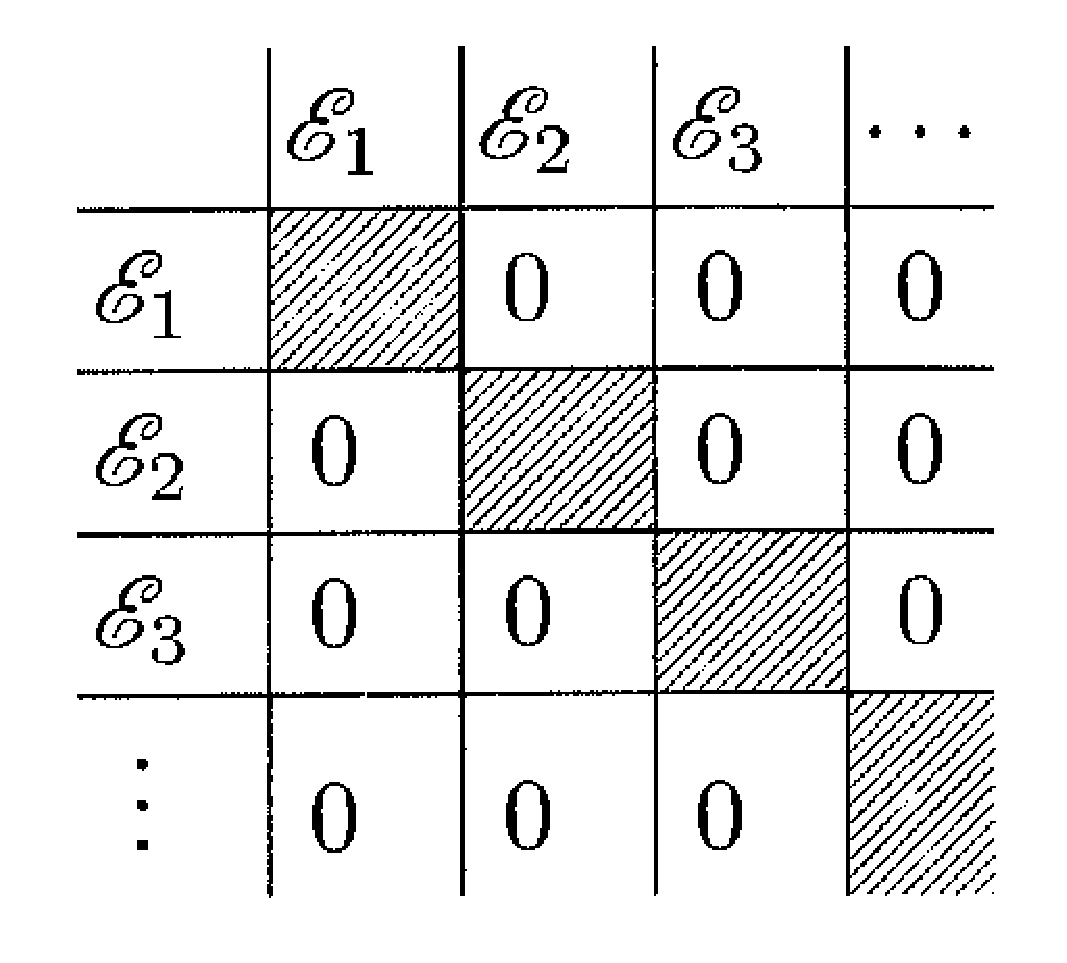
\includegraphics[scale=0.3]{fig/3-1.eps}
        \caption{$\hat{B}$的矩阵}
        \label{分块对角阵}
    \end{figure}
    \section{广义概率诠释}
    薛定谔只是捣鼓出来了一个波函数方程, 但全然不知波函数方程的物理意义是什么, 前面我们说了它的模方可以解释为粒子位置分布的概率密度函数, 这是广义解释的一个特例。
    \begin{proposition}{广义概率诠释}
        \setlength\parindent{2em}先考虑离散谱情况。我们对一个量子态$\Psi(x,t)$进行测量, 会得到观察算符$\hat{Q}$的一个本征值$q_n$, 而且因为测量, 体系会坍缩为$q_n$对应的一个本征态$\ket{\psi_n}$。
        且$\ket{\psi_n}$实际上是$\ket{\Psi}$在$q_n$所对应的本征空间的归一化投影。定义投影算符:
        \[P_n\equiv\sum\limits_{i=1}^{g_n} \ket{u_n^i} \bra{u_n^i}\]
        那么$\ket{\psi_n}$满足\footnote{利用了$P_n^2=P_n$}:
        \begin{equation}
            \ket{\psi_n}=\frac{P_n\ket{\Psi}}{\sqrt{\braket{\Psi|P_n|\Psi}}}
        \end{equation}
        \textbf{体系在测量之后会以$\ket{\psi_n}$为初态继续按照薛定谔方程演化}, 所以我们说测量一定会影响系统\footnote{但是对于一个本身就处于$\hat Q$的某个定值态的系统, 你测量$Q$并不会影响系统}。
        对这个系统测量, 得到$q_n$的概率为:
        \begin{equation}
            \mathscr{P}_n=\sum\limits_{i=1}^{g_n}\left|\Braket{u_n^i|\Psi}\right|
        \end{equation}
            
        
        \setlength\parindent{2em}对于连续谱, 我们前面提到过其本征矢是没有物理意义的, 也就是说, 进行测量时, 体系不会坍缩为一个确定的本征态, 而是一个很狭窄的
        范围, 因为只有这些本征矢组合成的波包才有确定的物理意义。

        \setlength\parindent{2em}对于非简并连续谱, 测量值在$\alpha\sim\alpha+\mathrm{d}\alpha$范围内的概率为:
        \begin{equation}
            \mathscr{P}(\alpha)\mathrm{d}\alpha=\left|c(\alpha)\right|^2\mathrm{d}\alpha,c(\alpha)=\left \langle u_\alpha  | \Psi  \right \rangle 
        \end{equation}
        这时, $\mathscr{P}(\alpha)$已经过渡为一个概率密度函数。

        \setlength\parindent{2em}至于连续非简并、部分连续部分离散等等情况都很容易依照上面的思路直接进行推广。
    \end{proposition}
    下面的叙述都以离散非简并情况为例, 对于一般情况也很好扩展。

    对于观察算符, 我们已经知道它的正交归一系是完备的, 所以态可以展开成:
    \[\left | \Psi  \right \rangle =\sum\limits_{n=1}^{\infty } c_n\left | u_n \right \rangle \]
    $c_n$就是态在某个本征态上的分量, 这样来看似乎前面的概率诠释也很有道理, 但是注意, 概率一定要取这个分量的模方。

    由于波函数在任何时间都是归一化的, 那么:
    \begin{equation*}
        1 = \left\langle {\Psi }
    \mathrel{\left | {\vphantom {\Psi  \Psi }}
    \right. \kern-\nulldelimiterspace}
    {\Psi } \right\rangle  = \left\langle \Psi  \right|\mathbbm{1}\left| \Psi  \right\rangle  = \sum\limits_n {\left\langle {\Psi }
    \mathrel{\left | {\vphantom {\Psi  {{u_n}}}}
    \right. \kern-\nulldelimiterspace}
    {{{u_n}}} \right\rangle \left\langle {{{u_n}}}
    \mathrel{\left | {\vphantom {{{u_n}} \Psi }}
    \right. \kern-\nulldelimiterspace}
    {\Psi } \right\rangle }  = \sum\limits_n {c_n^*{c_n} = } \sum\limits_n {{{\left| {{c_n}} \right|}^2}} 
    \end{equation*}
    从概率的角度看, 这个理论完全自洽。
    \begin{align*}
        \left\langle \Psi \right| \hat{Q}  \left| \Psi  \right\rangle & = \left\langle \Psi \right| \hat{Q} \mathbbm{1} \left| \Psi  \right\rangle = \sum_{n} \left\langle \Psi \right| \hat{Q} \left| u_n  \right \rangle\left \langle u_n  | \Psi  \right \rangle \\ 
        &=\sum_{n} q_n\left\langle  \Psi  |u_n  \right\rangle\left \langle u_n  | \Psi  \right \rangle\\
        &=\sum_{n} q_n\left| c_n \right| ^2\\
        &=\left\langle Q \right\rangle 
    \end{align*}
    我们得到了计算测量平均值的一般方法, 与前面提到的方法完全一致:
    \begin{equation}
        \label{eq:3.14}
        \boxed{\left\langle Q \right\rangle=\left\langle \Psi \right| \hat{Q}  \left| \Psi  \right\rangle}
    \end{equation}
    \begin{thinknote}
        \setlength\parindent{2em}前面已经算出了位置和动量算符的本征值及本征矢, 那么粒子位置的概率分布函数:
        \begin{align*}
            c\left ( y \right ) & = \left \langle g_y| \Psi  \right \rangle \\& = \int \Psi \left ( x,t \right ) \delta(x-y)\mathrm{d}x
            \\&=\Psi \left ( y,t \right ) 
        \end{align*}
        和波函数是完全一致的, 波尔概率诠释也就是这个内容。

        \setlength\parindent{2em}粒子动量的密度分布函数也可以计算出来:
        \begin{align*}
            c\left ( p \right ) & = \left \langle f_p  | \Psi  \right \rangle \\ & = \frac{1}{\sqrt{2\pi\hbar} } \int  \Psi(x,t)e^{-\frac{ipx}{\hbar } }\\
            &\equiv \Phi(p,t)
        \end{align*}
    \end{thinknote}
    这里引入了一个新的概念, \textbf{动量空间波函数}, $\Phi(p,t)$. 原先的$\Psi(x,t)$可以称为\textbf{位置空间波函数}。他们之间的关系就是傅里叶变换\footnote{量子力学里面更喜欢这样写傅里叶变换, 很容易证明它和我们之前讲自由粒子波函数时引进的傅里叶变换的等价性}:
    \begin{align}
        &\Phi(p,t)=\frac{1}{\sqrt{2\pi\hbar}}\int\Psi(x,t)e^{-\frac{ipx}{\hbar}}\mathrm{d}x\\
        &\Psi(x,t)=\frac{1}{\sqrt{2\pi\hbar}}\int\Phi(p,t)e^{\frac{ipx}{\hbar}}\mathrm{d}p
    \end{align}
    两个表示粒子状态的波函数都非常重要。
    \begin{proposition}{算符的两种不同形式}
        我们之前提到的$\hat x=x,\hat p=-i\hbar\frac{\partial}{\partial x}$实际上时算符在位置空间\footnote{暂时先这么说, 实际上应该说成$\left|\bm{r}\right\rangle$}下的描述, 在动量空间中应该是\footnote{为了和前面区分, 我改用$\tilde{}$表示算符}:
        \[\tilde{x}=i\hbar\frac{\partial}{\partial p},\tilde{p}=p\]
        或者更一般的, 使用两种不同空间波函数求力学量平均值应该写成:
        \begin{equation}
            \langle Q(x, p, t)\rangle=\left\{\begin{array}{ll}
                \int \Psi^{*} \hat{Q}\left(x,-i \hbar \frac{\partial}{\partial x}, t\right) \Psi d x, & \text { in position space; } \\
                \int \Phi^{*} \hat{Q}\left(i \hbar \frac{\partial}{\partial p}, p, t\right) \Phi d p, & \text { in momentum space. }
                \end{array}\right.
        \end{equation}
    \end{proposition}
    概率诠释是量子力学逻辑体系里面的一条基本假设, 这条假设之前的一个假设是我们上一节提到的, \textbf{每个可观测量对应一个观察算符}。
    \begin{thinknote}
        \textbf{例:证明对于定态(能量本征态), 有$\braket{p}=0$。}

        \flushleft{Proof:}

        \setlength\parindent{2em}首先通过计算可以得到下面的关系:
        \[\left[x,\hat{p}^2\right]=2i\hbar\hat p\Rightarrow\left[x,\hat H\right]=\frac{i\hbar}{m}\hat p\]
        利用广义概率诠释:
        \begin{align*}
            \braket{p}&=\Braket{\Psi|\hat p|\Psi}=\Braket{\psi|\hat p|\psi}\\
            &=\Braket{\psi|\frac{m}{i\hbar}\left[x,\hat H\right]|\psi}\\
            &=\frac{m}{i\hbar}\left(\Braket{\psi|x\hat H|\psi}-\Braket{\psi|\hat H x|\psi}\right)
        \end{align*}
        第一个等号的成立是因为$\ket{\Psi}$和$\ket{\psi}$只相差一个$\phi(t)$(而这个的本质是因为薛定谔方程的可分离变量性), 而且相位因子对平均值的计算没有影响。
        
        \setlength\parindent{2em}由于$\ket{\psi}$是能量本征态(严格来说应该是$\ket{\Psi}$, 但是相位因子对于定态问题真的没啥作用, 有没有这个相位因子都还是本征矢), 所以有:
        \[\hat H\ket{\psi}=E\ket{\psi}\]
        又因为$\hat H$是厄米算符, 而且$E\in\mathbbm{R}$, 所以上式取厄米共轭得:
        \[\bra{\psi}\hat H=\bra{\psi}E\]
        \begin{equation*}
            \braket{p}=\frac{m}{i\hbar}\left(\braket{\psi|xE|\psi}-\braket{\psi|Ex|\psi}\right)=0
        \end{equation*}
        \hfill $\square$\par
    \end{thinknote}
    \section{不确定性原理}
    在知晓广义概率诠释之后, 我们下面规定$\left\langle Q \right\rangle$, 即观测量的平均值, 有时也索性直接写成$\left\langle \hat Q \right\rangle$, 它
    和$\left\langle \Psi \right| \hat{Q}  \left| \Psi  \right\rangle$直接对应。后面的推导有时也不会严格使用狄拉克符号, 但请记住下面的转换关系:
    \[\left|\hat Q\Psi\right\rangle=\hat Q\left|\Psi\right\rangle, \left\langle \hat Q \Psi\right|=\left\langle \Psi\right|\hat{Q}^\dagger\]
    \begin{theorem}{不确定性原理}
        对于任意两个可观测量$\hat{A}, \hat{B}$, 对同一个系综测量后得到的方差总是满足下面的关系式:
        \begin{equation}
            \label{不确定性原理}
            \boxed{
                \sigma_A\sigma_B\geq\frac{1}{2}\left|\left\langle\left[\hat A,\hat B\right]\right\rangle\right|
            }
        \end{equation}
    \end{theorem}
    \begin{thinknote}
        Proof:
        \begin{align}
            &\sigma _A^2 = \left\langle {{\left( {\hat A - \left\langle A \right\rangle } \right)\Psi }}
            \mathrel{\left | {\vphantom {{\left( {\hat A - \left\langle A \right\rangle } \right)\Psi } {\left( {\hat A - \left\langle A \right\rangle } \right)\Psi }}}
            \right. \kern-\nulldelimiterspace}
            {{\left( {\hat A - \left\langle A \right\rangle } \right)\Psi }} \right\rangle  \equiv \left\langle {f}
            \mathrel{\left | {\vphantom {f f}}
            \right. \kern-\nulldelimiterspace}
            {f} \right\rangle \\
            &\sigma _B^2 = \left\langle {{\left( {\hat B - \left\langle B \right\rangle } \right)\Psi }}
            \mathrel{\left | {\vphantom {{\left( {\hat B - \left\langle B \right\rangle } \right)\Psi } {\left( {\hat B - \left\langle B \right\rangle } \right)\Psi }}}
            \right. \kern-\nulldelimiterspace}
            {{\left( {\hat B - \left\langle B \right\rangle } \right)\Psi }} \right\rangle  \equiv \left\langle {g}
            \mathrel{\left | {\vphantom {g g}}
            \right. \kern-\nulldelimiterspace}
            {g} \right\rangle 
        \end{align}
        根据Cauchy-Schwarz不等式, 可以得到:
        \[\sigma _A^2\sigma _B^2 = \left\langle {f}
        \mathrel{\left | {\vphantom {f f}}
        \right. \kern-\nulldelimiterspace}
        {f} \right\rangle \left\langle {g}
        \mathrel{\left | {\vphantom {g g}}
        \right. \kern-\nulldelimiterspace}
        {g} \right\rangle  \geqslant {\left| {\left\langle {f}
        \mathrel{\left | {\vphantom {f g}}
        \right. \kern-\nulldelimiterspace}
        {g} \right\rangle } \right|^2}\]
        任意复数可以拆分实部和虚部:
        \[{\left| {\left\langle {f}
        \mathrel{\left | {\vphantom {f g}}
        \right. \kern-\nulldelimiterspace}
        {g} \right\rangle } \right|^2} = {\left( {\operatorname{Re} \left\langle {f}
        \mathrel{\left | {\vphantom {f g}}
        \right. \kern-\nulldelimiterspace}
        {g} \right\rangle } \right)^2} + {\left( {\operatorname{Im} \left\langle {f}
        \mathrel{\left | {\vphantom {f g}}
        \right. \kern-\nulldelimiterspace}
        {g} \right\rangle } \right)^2} \geqslant {\left( {\operatorname{Im} \left\langle {f}
        \mathrel{\left | {\vphantom {f g}}
        \right. \kern-\nulldelimiterspace}
        {g} \right\rangle } \right)^2}\]
        \[\operatorname{Im} \left\langle {f}
        \mathrel{\left | {\vphantom {f g}}
        \right. \kern-\nulldelimiterspace}
        {g} \right\rangle  = \frac{{\left\langle {f}
        \mathrel{\left | {\vphantom {f g}}
        \right. \kern-\nulldelimiterspace}
        {g} \right\rangle  - \left\langle {g}
        \mathrel{\left | {\vphantom {g f}}
        \right. \kern-\nulldelimiterspace}
        {f} \right\rangle }}{{2\mathrm{i}}}\]
        \begin{align*}
            \left\langle {f}
            \mathrel{\left | {\vphantom {f g}}
            \right. \kern-\nulldelimiterspace}
            {g} \right\rangle  &= \left\langle {{\left( {\hat A - \left\langle A \right\rangle } \right)\Psi }}
            \mathrel{\left | {\vphantom {{\left( {\hat A - \left\langle A \right\rangle } \right)\Psi } {\left( {\hat B - \left\langle B \right\rangle } \right)\Psi }}}
            \right. \kern-\nulldelimiterspace}
            {{\left( {\hat B - \left\langle B \right\rangle } \right)\Psi }} \right\rangle  \\ 
                &= \left\langle {\Psi }
            \mathrel{\left | {\vphantom {\Psi  {\left( {\hat A - \left\langle A \right\rangle } \right)\left( {\hat B - \left\langle B \right\rangle } \right)\Psi }}}
            \right. \kern-\nulldelimiterspace}
            {{\left( {\hat A - \left\langle A \right\rangle } \right)\left( {\hat B - \left\langle B \right\rangle } \right)\Psi }} \right\rangle  \\ 
                &= \left\langle \Psi  \right|\hat A\hat B\left| \Psi  \right\rangle  - \left\langle A \right\rangle \left\langle \Psi  \right|\hat B\left| \Psi  \right\rangle  - \left\langle B \right\rangle \left\langle \Psi  \right|\hat A\left| \Psi  \right\rangle  + \left\langle A \right\rangle \left\langle B \right\rangle \left\langle {\Psi }
            \mathrel{\left | {\vphantom {\Psi  \Psi }}
            \right. \kern-\nulldelimiterspace}
            {\Psi } \right\rangle  \\ 
                &= \left\langle {\hat A\hat B} \right\rangle  - \left\langle A \right\rangle \left\langle B \right\rangle  \\ 
            \end{align*} 
        第二个等号成立是因为$\left\langle A \right\rangle \in \mathbbm{R}$且$\hat A$是厄米算符, 所以${\hat A - \left\langle A \right\rangle }$是厄米的。

        同理可得:
        \[\left\langle {g}\mathrel{\left | {\vphantom {g f}}\right. \kern-\nulldelimiterspace}{f} \right\rangle  = \left\langle {\hat B\hat A} \right\rangle  - \left\langle A \right\rangle \left\langle B \right\rangle \]
        结合上面的等式立即得到:
        \[\sigma _A^2\sigma _B^2 = {\left| {\frac{1}{{2i}}\left\langle {\left[ {\hat A,\hat B} \right]} \right\rangle } \right|^2}\]
        推导不确定性关系不需要额外的假设, 它可以看作是概率诠释和柯西不等式的一个推论。
        \hfill $\square$\par
    \end{thinknote}
    这个不等式中, 所谓的\uwave{不确定度}就蕴含在$\sigma$中, 它就表征了我们对一个系综测量, 整个测量结果的数据分散程度, 偏离平均值的程度。
    对于位置和动量之间的不确定性正是上面的普遍关系式的一个推论:
    \begin{equation}
        \label{x-p 不确定性}
        {\sigma _x}{\sigma _p} \geqslant \frac{1}{2}\left| {\left\langle {\left[ {\hat x,\hat p} \right]} \right\rangle } \right| = \frac{1}{2}\left| {\left\langle {i\hbar } \right\rangle } \right| = \frac{\hbar }{2}
    \end{equation}
    \begin{history}{海森堡对不确定性关系的理解}
        \setlength\parindent{2em}最初解释不确定性关系的时候, 海森堡总是认为它和测量是相关的, 因此有了个著名的思想实验。大致说的是当我们对一个电子进行测量时, 我们需要使用一个光子
        去撞击它, 也就是说会对它本身进行干扰, 我们对位置了解的越多, 那么我们对它的干扰也就越大, 我们对动量的了解程度就越少, 反之, 我们对动量了解的越多, 对
        位置信息了解的也越少了。
        
        \setlength\parindent{2em}这是海森堡当时对不确定性原理的解释, 因此不确定性原理也在上世纪常常被称为测不准原理, 事实上这个理解是很有问题的, 不确定性原理是量子力学不同于经典力学的
        一个原理, 是粒子本身的性质, 是一个普遍物理规律, 和你是否进行测量是毫无关系的。
    \end{history}
    在前面我们证明过, 两个可对易观察算符可以同时对角化。我们称在这两个\textbf{可观测量是相容的}, 从不确定性原理的角度理解就是这两个观测量是可以同时测量的。
    测量两个量的顺序是无关紧要的, 测量$A$之后测量$B$也不会让第一次测量的信息得到损失, 反而会得到补充, 这一切的一切定性点来看就是两次坍缩得到的本征态同时是两个
    算符的本征态。仔细分析有点复杂, 可以参考科恩第三章$\S B$。

    我们再来看一下不等式\ref{不确定性原理}等号成立的\uwave{必要条件}:
    \[g = cf \wedge \operatorname{Re} \left\langle {f}\mathrel{\left | {\vphantom {f g}}\right. \kern-\nulldelimiterspace}{g} \right\rangle  = 0,c\in \mathbbm{C}\]
    根据内积的正定性, 直接得到$c$是一个纯虚数, 我们记作$\mathrm{i}a$, 其中$a\in\mathbbm{R}$

    回到动量位置不确定性关系上来, 如果式\ref{x-p 不确定性}可以取等号, 那么根据前面分析
    \[\left( {\hat p - \left\langle p \right\rangle } \right)\Psi  = ia\left( {\hat x - \left\langle x \right\rangle } \right)\Psi  \Rightarrow \left( { - i\hbar \frac{d}{{dx}} - \left\langle p \right\rangle } \right)\Psi  = ia\left( {x - \left\langle x \right\rangle } \right)\Psi \]
    解微分方程得到波函数的形式是\footnote{$\left\langle x \right\rangle,\left\langle p \right\rangle$和位置$x$无关。}:
    \begin{equation}
        \Psi  = A{e^{ - \frac{a}{{2\hbar }}{{\left( {\hat x - \left\langle x \right\rangle } \right)}^2}}}{e^{\frac{i}{\hbar }\left\langle p \right\rangle x}}
    \end{equation}
    这显然是一个高斯分布的形式。当然, 只是当某个时刻波函数有这个形式时式\ref{x-p 不确定性}取等号, 之后波函数随时间演化后可能就不再满足取等条件了。
    \subsection*{时间能量不确定性关系}
    很多书籍把不确定性关系也写作
    \begin{equation}
       \Delta {x} \Delta {p} \ge \frac{\hbar}{{2 }} 
    \end{equation}
    对应的还会有一个时间和能量之间的不确定性关系\footnote{从狭义相对论动力学的四位动量和四维时空坐标中你可以看出这种对应性}:
    \begin{equation}
        \label{E-t}
        \Delta {t} \Delta {E} \ge \frac{\hbar}{{2 }}
    \end{equation}
    
    
    这两个公式看起来非常相似, 但是物理实质却有很大的区别, 从$\Delta t$就可以看出来。难道指的是时间的标准差?时间只是演化之中的一个参数而已, 何来标准差一说。
    所以从我们下面的推导中, 要格外注意两个公式的不同之处。
    \begin{equation}
        \label{求导式子}
        \frac{d}{d t}\langle Q\rangle=\frac{d}{d t}\langle\Psi|\hat{Q}| \Psi\rangle=\Braket{\frac{\partial \Psi}{\partial t}|\hat{Q}| \Psi}+\Braket{\Psi|\frac{d \hat{Q}}{d t}|\Phi}+\Braket{\Psi|\hat{Q}| \frac{\partial \Psi}{\partial t}}
    \end{equation}
    上面的求导具体过程可以使用定义直接推导, 有点像实分析中三个函数相乘的导数公式。\footnote{$\Ket{\frac{\partial \Psi}{\partial t}}$表示$\frac{\partial }{\partial t}\Ket{\Psi}$, 对应的左矢为$\Bra{\frac{\partial \Psi}{\partial t}}$, 注意不是$\frac{\partial }{\partial t}\Bra{\Psi}$}
    
    含时薛定谔方程可以写为\footnote{严格使用狄拉克符号的话这里的$\Psi$要加上$\ket{}$}:
    \[i\hbar\frac{\partial \Psi}{\partial t}=\hat H\Psi\Rightarrow\frac{\partial \Psi}{\partial t}=-\frac{i\hat H}{\hbar}\Psi\]
    代入\ref{求导式子}得到:
    \begin{align*}
        \frac{d\braket{Q}}{dt}&=\Braket{\frac{\hat{H}}{i\hbar}\Psi |\hat{Q}|\Psi}+\Braket{\Psi|\frac{\partial \hat{Q}}{\partial t}|\Psi}+\Braket{\Psi|\hat{Q}| \frac{\hat H}{i\hbar}\Psi}\\
        &=\frac{i}{\hbar}\Braket{\Psi|\hat H\hat Q|\Psi}+\Braket{\Psi|\frac{\partial \hat{Q}}{\partial t}|\Psi}-\frac{i}{\hbar}\Braket{\Psi|\hat Q\hat H|\Psi}\\
        &=\frac{i}{\hbar}\Braket{\Psi|\left[\hat H,\hat Q\right]|\Psi}+\Braket{\frac{\partial \hat Q}{\partial t}}
    \end{align*}
    也就是说对于任何的可观测量, 我们可以得到它的平均值随时间变化的规律, 是与体系的哈密顿算符(量)之间相关的:
    \begin{equation}
        \label{广义欸费斯托定理}
        \boxed{
            \frac{d\braket{Q}}{dt}=\frac{i}{\hbar}\Braket{\Psi|\left[\hat H,\hat Q\right]|\Psi}+\Braket{\frac{\partial \hat Q}{\partial t}}
        }
    \end{equation}
    当\ref{广义欸费斯托定理}中的$\hat Q=\hat p$时\footnote{我们目前的讨论都在位置空间中, 所以$\hat p=-i\hbar\frac{\partial}{\partial x}$}, 我们得到\textbf{Ehrenfest's theorem}:
    \begin{equation}
        \boxed{\frac{d}{dt}\braket{p}=\Braket{-\frac{\partial V(x)}{\partial x}}}
    \end{equation}

    一般来说, 很多算符都是不显含时间的, 与时间无关, 我们着重研究这些算符, 式\ref{广义欸费斯托定理}写成:
    \[\frac{d\braket{Q}}{dt}=\frac{i}{\hbar}\Braket{\Psi|\left[\hat H,\hat Q\right]|\Psi}\]
    又因为$\hat{H}$和$\hat{Q}$都是两个可观测量, 那么由不确定性原理有:
    \[\sigma_H\sigma_Q\geq\frac{1}{2}\left|\Braket{\left[\hat H,\hat Q\right]}\right|\]
    联立以上两式, 得:
    \begin{equation}
        \label{H-Q}
        \sigma_H\sigma_Q\geq\frac{\hbar}{2}\left|\frac{d\braket{Q}}{dt}\right|
    \end{equation}
    由于哈密顿量对应的是体系的能量, 所以我们把$\sigma_H$记作$\Delta E$, 为了凑出不确定性原理, 我们\textbf{定义}$\Delta t$为:
    \begin{equation}
        \label{define dt}
        \sigma_Q=\left|\frac{d\braket{Q}}{dt}\right|\Delta t
    \end{equation}
    
    它确实具有时间量纲, 可见这个时候, \ref{E-t}和我们关注的可观测量是相关的。按照上面的公式你可以严格去验证不确定性原理, 但是这通常很麻烦, 借用计算机方面的
    一个词语, \textbf{时间能量不确定性关系又很好的鲁棒性}。所以我们一半对于$\Delta t$的解释很随意, 用来进行一些估算是很好的, 根据$\Delta t$的定义, 其实我们也有理由
    说:\textbf{\textcolor{red}{$\Delta t$可以解释为系统产生一个“显著”的变化所需要的时间}}。
    \begin{thinknote}
        “显著”变化的时间, 这个论述就非常的缺乏严谨性, 非常模棱两可。所以这个不等式中的$\Delta t$在很多情况下都有非常“物理”的解释, 可以说通, 但比不上式\ref{define dt}的
        严谨性, 很多时候这个式子用来估算非常好, 这方面的例子{\itshape Griffiths}书里面有三个。
    \end{thinknote}
    \section{表象理论}
    {\itshape Griffiths}书里面的这一节的绝大部分内容在附录\ref{Appendix B}中已讲, 这里我们回到{\itshape Cohen}第二章, 给狄拉克符号相关内容结尾。
    
    在附录\ref{Appendix B}中我们最先研究了波函数空间$\mathscr{F}$, 这里的波函数指的是以坐标为参数表示的波函数, 可以用波函数表示一个量子态。但是实际上我们发现量子态更本质上可以
    使用态矢量来描述, 我们便引进了$\mathscr{E}_r$空间, 实际上你可以认为波函数空间中的元素就是对应态空间矢量在\uwave{位置表象}下的分量函数。实际上, 量子力学的一个基本假设就是任何一个体系的
    量子态可以使用态空间中的一个右矢表示, 在附录\ref{Appendix B}中我们已经讨论了这个空间的运算性质, 其代数本质是线性空间, 下面我们正式从$\mathscr{F}$空间定义与其联系的$\mathscr {E}_r$空间, 其实就是一个
    通过分量和一组完备的正交基确定矢量的过程。
    \begin{proposition}{$\mathscr{F}$空间与$\mathscr {E}_r$空间的联系}
        对于波函数空间中的每一个波函数$\psi(bm{r})$, 我们唯一选取态空间中的一个右矢$\ket{\psi}$与之对应, 这种对应是线性的, 而且这种对应使得内积定义为\footnote{我们正是在定义一个内积空间}:
        \begin{equation}
            \label{eq:3.30}
            \braket{\varphi|\psi}=\int d^3r\varphi^*(\bm{r})\psi(\bm{r})
        \end{equation}
    \end{proposition}
    我们下面的讨论直接使用三维形式, 实际上就是每个维度的缩并形式。
    \subsection*{$\ket{\bm{r}}$和$\ket{\bm{p}}$表象}
    波函数空间中可以找到两组不属于$\mathscr{F}$的基, 满足封闭性关系和狄拉克正交归一关系:
    \begin{align}
        \label{eq:3.31}& \xi_{\bm{r}_0}(\bm{r})=\delta({\bm{r}-\bm{r}_0})\\
        \label{eq:3.32}& \nu_{\bm{p}_0}(\bm{r})=\left(2\pi\hbar\right)^{-\frac{3}{2}}e^{\frac{i}{\hbar}\bm{p}_0\cdot\bm{r}}
    \end{align}
    
    我们可以给这两个波函数分别对应两个\uwave{广义右矢}$\ket{\bm{r}_0},\ket{\bm{p}_0}$。再根据\ref{eq:3.30}我们可以得出态矢量$\Ket{\Psi}$在这两组基下的分量:
    \begin{align}
        &\Braket{\bm{r}_0|\Psi}=\Psi(\bm{r}_0)\\
        &\Braket{\bm{p}_0|\Psi}=\mathscr{F}\left[\Psi(\bm{r})\right](\bm{p}_0)=\Phi(\bm{p}_0)
    \end{align}
    可见态矢量在$\ket{\bm{r}}$上的分量正是波函数在这个指标下的取值。我们将$\ket{\bm{r}_0}$换成$\ket{\bm{r}}$, 那么内积得到的就是一个关于$\ket{\bm{r}}$
    的函数, 也正是波函数本身。我们将上式写成下面更紧凑的形式, 方便我们看清之前定义的位置空间波函数和动量空间波函数的意义:
    \begin{align}
        &\braket{\bm{r}|\Psi}=\Psi(\bm{r})\Rightarrow \ket{\Psi}=\int d^3r \ket{\bm{r}}\braket{\bm{r}|\Psi}=\int d^3r \Psi(\bm{r})\ket{\bm{r}}\\
        &\braket{\bm{p}|\Psi}=\Phi(\bm{p})\Rightarrow \ket{\Psi}=\int d^3p \ket{\bm{r}}\braket{\bm{p}|\Psi}=\int d^3p \Phi(\bm{p})\ket{\bm{p}}
    \end{align}
    实际上, 任何一个可观测量对应的观察算符的特征矢都可以组成一个规范正交基(满足\ref{eq:B.12}和\ref{eq:B.13}), 也就确定了一个表象。比如同样经常用的能量表象, 就是根据
    哈密顿算符定义的, 也就是我们第二章一直在求的定态解$\ket{\psi}$, 他们也可以构成一个基底, 对于束缚态同样可以写:
    \[\ket{\Psi}=\sum\limits_n c_n\ket{\psi_n}\]  
    如果量子态$\ket{\Psi}$随时间演化, 那么上面的分量波函数或者是$c_n$都要带上时间参量, 基底还是一般不用随时变的。
    
    根据式\ref{eq:3.31}和式\ref{eq:3.32}, 我们可以得到\[\braket{\bm{r}|\bm{p}}=\left(2\pi\hbar\right)^{-\frac{3}{2}}e^{\frac{i}{\hbar}\bm{p}\cdot\bm{r}}\]
    使用附录B中类似的方法, 可以得到表象之间的变换关系:
    \begin{align*}
        \Phi(\bm{r})&=\Braket{\bm{r}|\Psi}=\Braket{\bm{r}|\mathbbm{1}|\Psi}\\
        &=\int d^3p\Braket{\bm{r}|\bm{p}}\Braket{\bm{p}|\Psi}=\int d^3p\left(2\pi\hbar\right)^{\frac{3}{2}}e^{\frac{i}{\hbar}\bm{p}_0\cdot\bm{r}}\Phi(\bm{p})\\
        &=\mathscr{F}^{-1}\left[\Phi(\bm{p})\right](\bm{r})
    \end{align*}
    我们使用了一种新的方式去说明两种波函数之间的傅里叶变换关系, 当然, 这里的傅里叶变换是一个三维形式。
    \subsection*{算符$\hat{\bm{R}}$和算符$\hat{\bm{P}}$}
    下面我们要讨论的可以看作是$\hat x$和$\hat p$的三维形式。
    \begin{define}{两个重要算符}
        \begin{itemize}
            \item 算符$\hat{\bm{R}}$\\
            这个算符在$\ket{\bm{r}}$表象下由三个“分量算符”$X,Y,Z$确定。\footnote{这里的$\bm{r}$是个缩并的记号, 波函数实际上是一个三元函数$\Psi(x,y,z)$, 下式中的$x,y,z$就是包含在$\ket{\bm{r}}$中的三个指标。算符$\hat{\bm{P}}$同理。}
            \begin{align*}
                &\Braket{\bm{r}|X|\Psi}=x \Braket{\bm{r}|\Psi}=x\Psi(\bm{r})\\
                &\Braket{\bm{r}|Y|\Psi}=y \Braket{\bm{r}|\Psi}=y\Psi(\bm{r})\\
                &\Braket{\bm{r}|Z|\Psi}=z \Braket{\bm{r}|\Psi}=z\Psi(\bm{r})
            \end{align*}
            \item 算符$\hat{\bm{P}}$\\
            这个算符在$\ket{\bm{p}}$表象下由三个“分量算符”$P_x,P_y,P_z$确定。\footnote{如果考虑随时间演化的态, 式中要加上时间项, 形式不变。}
            \begin{align*}
                &\Braket{\bm{p}|P_x|\Psi}=p_x \Braket{\bm{p}|\Psi}=p_x\Phi(\bm{p})\\
                &\Braket{\bm{p}|P_y|\Psi}=p_y \Braket{\bm{p}|\Psi}=p_y\Phi(\bm{p})\\
                &\Braket{\bm{p}|P_z|\Psi}=p_z \Braket{\bm{p}|\Psi}=p_z\Phi(\bm{p})
            \end{align*}
        \end{itemize}
    \end{define}
    那么根据上面的定义, 就可以解释我们一直说的在位置空间中$\hat{x}\leftrightarrow x$, 换成矩阵的语言, 就是在位置表象下, 算符$\hat{x}$的矩阵是$x\mathbbm{1}$, 因为波函数完全可以看作一个列矩阵。
    两者相乘便得到了$\hat{x}\ket{\psi}$在位置表象下的形式(波函数)。

    我们来看一下动量算符在位置表象下的形式, 我们不去直接计算矩阵元, 先将它作用于一个右矢再取分量可以很快的看出它的等价形式:
    \begin{align*}
        \Braket{\bm{r}|P_x|\Psi}&=\int d^3p\Braket{\bm{r}|\bm{p}}\Braket{\bm{p}|P_x|\Psi}=\int d^3pp_x\Braket{\bm{r}|\bm{p}}\Braket{\bm{p}|\Psi}\\
        &=\int d^3pp_x\left(2\pi\hbar\right)^{-\frac{3}{2}}e^{\frac{i}{\hbar}\bm{p}\cdot\bm{r}}\Phi(\bm{p})\\
        &=-i\hbar\frac{\partial}{\partial x}\int d^3p\left(2\pi\hbar\right)^{-\frac{3}{2}}e^{\frac{i}{\hbar}\bm{p}\cdot\bm{r}}\Phi(\bm{p})\\
        &=-i\hbar\frac{\partial}{\partial x}\Psi(\bm{r})
    \end{align*}
    所以在位置空间中$\hat p\leftrightarrow -i\hbar\frac{\partial}{\partial x}$, 进一步写成缩并形式便有:
    \begin{equation}
        \Braket{\bm{r}|\hat{\bm{P}}|\Psi}=-i\hbar\nabla\Braket{\bm{r}|\Psi}
    \end{equation}
    
    式\ref{eq:3.14}, 告诉了我们计算物理量平均值的办法, 实际上我们一般用的都是它在位置或动量空间下的形式, 严格点说, 式\ref{eq:3.14}可以利用封闭性关系重新写成
    \[\Braket{Q}=\int d^3r\Braket{\Psi|\bm{r}}\Braket{\Psi|\hat Q}|\Psi\]
    再利用上面已经得出的动量和位置算符在位置空间中的表示替换上式中的第二项即可, 也就是第一章就说的“把算符夹在中间, 然后积分”。

    很容易证明, $\ket{\bm{r}}$和$\ket{\bm{p}}$分别是$\hat {\bm{R}}$和$\hat {\bm{P}}$的本征矢。
    \subsection*{力学量完全集(CSCO)}
    对于某个观察算符$\hat{A}$, 可以选取一组它的正交归一本征矢$\{\ket{u^i_n}\}$作为$\mathscr{E}$中的一组基。如果对于$\hat A$的每一个本征值都是非简并的, 那
    么, 给定了$\hat{A}$的本征值也就唯一确定了这个正交归一基$\{\ket{u_n}\}$(显然这个时候我们不再需要额外使用指标$i$去区分), 因为每个本征子空间$\mathscr{E}_n$的维数都是一, 我
    们认为成比例的两个基矢是没有区别的, 即$\ket{u_n}\leftrightarrow e^{i\theta}\ket{u_n}$。这个时候我们就称算符$\hat{A}$单独构成了一个CSCO。
    
    如果存在一些非简并的本征值, 那么这个时候$\mathscr{E}_n$中本征矢的取法就有无限多种线性组合, 那么$\{\ket{u_n^i}\}$的取法就并不唯一了, 但我们这个时候如果引进一个
    与$\hat{A}$对易的算符$\hat{B}$, 考察他们的公共本征矢, 根据$\S{3.2}$的推导, 他们的公共本征矢构成了一组基$\{\ket{u_{n,p}^i}\}$, 由$\hat{A},\hat{B}$的本征矢对$\left(a_n,b_p\right)$确定。
    如果每一个本征矢对唯一确定了一个$\{\ket{u_{n,p}^i}\}$(同样, 成比例算作相同的本征矢), 那么$\hat{A},\hat{B}$的公共本征矢确定的基底是唯一的\footnote{根据$\S{3.2}$构造这组基的过程
    , 可以发现, 这个条件等价于${\left. {\hat B} \right|_{\mathscr{E}_n}}$(也就是那每一个分块小矩阵)有$g_n$个不同的本征值, 其中$g_n\equiv \dim \mathscr{E}_n$}, 这时我们称$\{\hat{A},\hat{B}\}$
    构成了一个CSCO。
    
    如果这个时候对于每个本征矢对还是无法唯一确定一个本征矢, 那么我们可以引进第三个同时与$\hat A,\hat B$对易的算符$\hat C$, 再次按照前面的情况分类讨论, 一般的CSCO定义如下:
    \begin{define}{力学量完全集(CSCO)}
        \setlength\parindent{2em}按定义, 把观察算符$\hat A,\hat B,\hat C\cdots$的一个集合叫做可对易观察算符的完全集合的条件是:
        \begin{itemize}
            \item 所有的这些观察算符\uwave{两两对易};
            \item 给出了全体算符$\hat A,\hat B,\hat C\cdots$的本征值的一个数组,便足以决定唯一的一个共同本征矢\footnote{有且仅有($\exists!$)}(倍乘因子除外)。
        \end{itemize}
        \setlength\parindent{2em}或者说:存在着由共同本征矢构成的一个正交归一基,而且这个基是唯一的(除相位因子以外)。
    \end{define}
    比如三维问题中$\hat{bm{R}}$算符的三个分量算符$X,Y,Z$就构成了一个CSCO, 很容易证明它们两两对易, 而且给定了本征值$(x_0,y_0,z_0)$就唯一确定了本征矢$\ket{\bm{r}}$, 显然这正是$\ket{\bm{r}}$表象。

    \section{薛定谔方程的分离变量}
    第二章中我们直接从波函数出发, 给出了很多结论, 实际上现在看来就是一些更广泛的结论在位置表象下的描述。比如我们第二章都是分离变量先解出定态解, 然后说明波动方程
    的通解是这些定态解的线性组合。现在我们知道这些定态解就是哈密顿算符的本征矢(用$\ket{\psi_n}$表示), 哈密顿算符是一个观察算符, 显然这些本征矢构成了一组基, 那么态矢量显然就可以用这组基底表示(以离散谱为例):
    \begin{equation}
        \label{eq:3.38}
        \Ket{\Psi(t)}=\sum_n c_n(t)\ket{\psi_n}
    \end{equation}
    
    但是这远远不够, 显然, 我们如果不对$c_n$加以限制的话, 式\ref{eq:3.38}实际上可以表示态空间的所有矢量!真正满足量子力学规律的矢量显然有一定限制, 而这个限制就是通过薛定谔方程和$\ket{\psi_n}$对应的本征值完成的。
    实际上之前我们利用分离变量法求解薛定谔方程(哈密顿量不显含时间, 即保守体系)就已经得出了$c_n$要满足的规律(式\ref{find_c}), 即\[c_n(t)=c_n(0) e^{-iE_n t/\hbar}\]
    下面我们全程使用更广泛的狄拉克符号法来推导一下\footnote{这里作为例子考虑最简单的离散谱非简并情况, 其他情况的推广非常简单}。
    
    我们之前解的薛定谔方程都是下面更加普遍的方程在$\ket{\bm{r}}$表象下的形式:
    \begin{lequation}
        \label{eq:3.39}
        i\hbar\frac{\partial}{\partial t}\ket{\Psi(t)}=\hat{H}\ket{\Psi(t)}
    \end{lequation}
    定态方程可以写为:
    \begin{lequation}
        \hat{H}\ket{\psi_n}=E_n\ket{\psi_n}\Rightarrow\bra{\psi_n}\hat{H}=E_n\bra{\psi_n}
    \end{lequation}
    在能量表象下, \ref{eq:3.39}变为:
    \[i\hbar\Braket{\psi_n|\frac{\partial}{\partial t}|\Psi(t)}=\Braket{\psi_n|\hat{H}|\Psi(t)}\]
    又因为$\ket{\psi_n}$与时间无关\footnote{因为$\hat H$不显含时间, 我们始终可以选取一组与时间无关的定态作为基底}, 那么上式又可以写为:
    \begin{align*}
        i\hbar\frac{\partial}{\partial t}\Braket{\psi_n|\Psi(t)}&=\Braket{\psi_n|\hat{H}|\Psi(t)}\\
        &=E_n\Braket{\psi_n|\Psi(t)}
    \end{align*}
    \[i\hbar\frac{d}{dt}c_n(t)=E_n c_n(t)\]
    对时间积分得到:
    \[c_n(t)=c_n(t_0)e^{-iE_n(t-t_0)/\hbar}\]
    为了方便, 有时我们从初态开始计时,$t_0=0$, 方程也就变成了我们经常看见的\ref{wiggle-function}。

    所以, 要计算态随时间的演化, 我们先解出系统的能量本征态(定态), 然后根据初态对能量表象展开计算出对应的$c_n(t_0)$
    $$c_n(t_0)=\Braket{\psi_n|\Psi(t_0)}$$
    然后再对于每个$c_n$乘上对应的波动项即可:
    \begin{equation}
        \ket{\Psi(t)}=\sum_n c_n(t_0)e^{-iE_n(t-t_0)/\hbar}\ket{\psi_n}
    \end{equation}

    这里再次强调一下, 按照上面的做法, 可以发现定态, 即能量本征态随时间的演化始终只是乘上一个$e^{i\theta}$, 而我们提到过这种成比例的态在物理上是不可区分的, 所以
    定态的一切物理性质都不会随时间改变。而其它的算符对应的定值态就不一定有这样的性质了, 只是每次对相应力学量的测量都返回同一个值(这个本征态对应的本征值), 而不像定态一样是所有物理性质不随时变。
